%=======================================================================
%  IE 5311-001 (D01) Principles of Optimization
%  Homework 04 solutions
%
%  Packages: geometry, amsmath, amssymb, amsthm, booktabs, array,
%  graphicx. All ship with Overleaf and with a full TeX Live install.
%  The figure p4_cone.pdf is produced by p4_cone.py and must sit beside
%  this file; the include is guarded, so the document builds without it.
%=======================================================================
\documentclass[11pt]{article}

\usepackage[margin=1in]{geometry}
\usepackage{amsmath}
\usepackage{amssymb}
\usepackage{amsthm}
\usepackage{booktabs}
\usepackage{array}
\usepackage{graphicx}

\DeclareMathOperator{\Aff}{Aff}
\DeclareMathOperator{\cone}{cone}
\DeclareMathOperator{\conv}{conv}
\DeclareMathOperator{\spn}{span}
\DeclareMathOperator{\rec}{rec}
\DeclareMathOperator{\Proj}{Proj}
\DeclareMathOperator{\dimop}{dim}
\DeclareMathOperator*{\minimize}{min}

\theoremstyle{definition}
\newtheorem*{definition}{Definition}
\newtheorem{remark}{Remark}
\theoremstyle{plain}
\newtheorem{proposition}{Proposition}
\newtheorem{lemma}{Lemma}

\setlength{\parskip}{0.45em}
\setlength{\parindent}{0pt}

\begin{document}

\begin{center}
  {\large IE 5311-001 (D01) Principles of Optimization}\\[4pt]
  Lidivine Kengne\\[2pt]
  Homework 04
\end{center}
\vspace{0.6em}

%=======================================================================
\section*{Problem 1.\quad Affine independence \quad[15 pts]}
%=======================================================================

Throughout, $\{v_i\}_{i \in [n]}$ is a finite family in a real vector
space, and
\[
  \Aff(S) \;:=\;
  \Big\{ \textstyle\sum_{j} \mu_j w_j \;:\;
    w_j \in S,\; \mu_j \in \mathbb{R},\;
    \textstyle\sum_j \mu_j = 1 \Big\}
\]
is the set of affine combinations of $S$. The three statements are

\begin{enumerate}
  \item[(1)] $v_i \notin \Aff(\{v_j\}_{j \ne i})$ for all $i \in [n]$;
  \item[(2)] $\sum_{i \in [n]} \lambda_i v_i = 0$ and
        $\sum_{i \in [n]} \lambda_i = 0$ imply $\lambda_i = 0$ for all
        $i \in [n]$;
  \item[(3)] $\{v_i - v_n\}_{i \in [n-1]}$ are linearly independent.
\end{enumerate}

We prove the cycle $(1) \Rightarrow (2) \Rightarrow (3) \Rightarrow (1)$,
which gives all three equivalences.

One substitution is used twice, so we record it first.

\begin{lemma}\label{lem:sub}
Let $\lambda_1,\dots,\lambda_n \in \mathbb{R}$ with
$\sum_{i \in [n]} \lambda_i = 0$. Then
\[
  \sum_{i \in [n]} \lambda_i v_i
  \;=\; \sum_{i \in [n-1]} \lambda_i\,(v_i - v_n).
\]
\end{lemma}

\begin{proof}
From $\sum_{i \in [n]} \lambda_i = 0$ we get
$\lambda_n = -\sum_{i \in [n-1]} \lambda_i$. Hence
\[
  \sum_{i \in [n]} \lambda_i v_i
  = \sum_{i \in [n-1]} \lambda_i v_i + \lambda_n v_n
  = \sum_{i \in [n-1]} \lambda_i v_i
    - \Big( \sum_{i \in [n-1]} \lambda_i \Big) v_n
  = \sum_{i \in [n-1]} \lambda_i (v_i - v_n). \qedhere
\]
\end{proof}

\subsection*{1.\quad $(1) \Rightarrow (2)$}

\begin{proof}
By contraposition. Suppose (2) fails: there are scalars
$\lambda_1,\dots,\lambda_n$, \emph{not all zero}, with
\[
  \sum_{i \in [n]} \lambda_i v_i = 0
  \qquad\text{and}\qquad
  \sum_{i \in [n]} \lambda_i = 0 .
\]
Choose $k$ with $\lambda_k \ne 0$. Solving the first equation for $v_k$
and dividing by $\lambda_k$,
\[
  v_k \;=\; \sum_{j \ne k} \Big( \frac{-\lambda_j}{\lambda_k} \Big) v_j .
\]
The coefficients sum to one: since $\sum_{i \in [n]} \lambda_i = 0$ we
have $\sum_{j \ne k} \lambda_j = -\lambda_k$, so
\[
  \sum_{j \ne k} \frac{-\lambda_j}{\lambda_k}
  = \frac{-1}{\lambda_k} \sum_{j \ne k} \lambda_j
  = \frac{-1}{\lambda_k}\,(-\lambda_k) = 1 .
\]
Hence $v_k$ is an affine combination of $\{v_j\}_{j \ne k}$, that is
$v_k \in \Aff(\{v_j\}_{j \ne k})$, so (1) fails.
\end{proof}

\subsection*{2.\quad $(2) \Rightarrow (3)$}

\begin{proof}
Assume (2). Let $\mu_1,\dots,\mu_{n-1} \in \mathbb{R}$ satisfy
\[
  \sum_{i \in [n-1]} \mu_i (v_i - v_n) = 0 .
\]
Define $\lambda_i := \mu_i$ for $i \in [n-1]$ and
$\lambda_n := -\sum_{i \in [n-1]} \mu_i$. Then
$\sum_{i \in [n]} \lambda_i = 0$ by construction, and by
Lemma~\ref{lem:sub},
\[
  \sum_{i \in [n]} \lambda_i v_i
  = \sum_{i \in [n-1]} \lambda_i (v_i - v_n)
  = \sum_{i \in [n-1]} \mu_i (v_i - v_n) = 0 .
\]
So $(\lambda_i)$ satisfies both hypotheses of (2), giving
$\lambda_i = 0$ for every $i$; in particular $\mu_i = \lambda_i = 0$ for
all $i \in [n-1]$. Hence $\{v_i - v_n\}_{i \in [n-1]}$ is linearly
independent.
\end{proof}

\subsection*{3.\quad $(3) \Rightarrow (1)$}

\begin{proof}
Assume (3) and suppose, for contradiction, that (1) fails: there is an
index $k$ and scalars $(\mu_j)_{j \ne k}$ with
\[
  v_k = \sum_{j \ne k} \mu_j v_j,
  \qquad \sum_{j \ne k} \mu_j = 1 .
\]
Set $\lambda_k := -1$ and $\lambda_j := \mu_j$ for $j \ne k$. Then
\[
  \sum_{i \in [n]} \lambda_i = 1 - 1 = 0,
  \qquad
  \sum_{i \in [n]} \lambda_i v_i = \sum_{j \ne k} \mu_j v_j - v_k = 0 .
\]
By Lemma~\ref{lem:sub} the second identity becomes
$\sum_{i \in [n-1]} \lambda_i (v_i - v_n) = 0$, so (3) forces
$\lambda_i = 0$ for all $i \in [n-1]$, and then
$\lambda_n = -\sum_{i \in [n-1]} \lambda_i = 0$ as well. Every
$\lambda_i$ vanishes, contradicting $\lambda_k = -1 \ne 0$. Hence (1)
holds.
\end{proof}

The cycle is closed, so (1), (2) and (3) are equivalent. $\blacksquare$

\begin{remark}
Statement (3) singles out $v_n$, but (2) treats the indices
symmetrically, so by the equivalence the choice of which point to
subtract is immaterial: $\{v_i - v_k\}_{i \ne k}$ is linearly
independent for one $k$ if and only if it is for every $k$.
\end{remark}

%=======================================================================
\section*{Problem 2.\quad Preimages under an affine map \quad[15 pts]}
%=======================================================================

\subsection*{1.\quad $f^{-1}(U)$ is convex}

\begin{proof}
If $f^{-1}(U) = \emptyset$ it is convex vacuously, so assume it is
nonempty and take $x, y \in f^{-1}(U)$ and $\theta \in [0,1]$.

Because $f$ is affine it preserves affine combinations, and a convex
combination is an affine combination, so
\[
  f\big( \theta x + (1-\theta) y \big)
  \;=\; \theta f(x) + (1-\theta) f(y) .
\]
By assumption $f(x) \in U$ and $f(y) \in U$, and $U$ is convex, so the
right-hand side lies in $U$. Therefore
$f(\theta x + (1-\theta)y) \in U$, which is exactly
$\theta x + (1-\theta) y \in f^{-1}(U)$.
\end{proof}

\subsection*{2.\quad The concrete map}

Here $\mathcal{V} = \mathbb{R}^m$, $\mathcal{W} = \mathbb{R}^n$ with
$m > n$, $f(v) = Av + a$, and $A \in \mathbb{R}^{n \times m}$ has
$A_{ii} = 2^i$ for $i \in [n]$ and every other entry zero. In block
form
\[
  A \;=\; \begin{bmatrix} D & 0 \end{bmatrix},
  \qquad
  D = \operatorname{diag}\big(2^1, 2^2, \dots, 2^n\big)
    \in \mathbb{R}^{n \times n},
\]
with $0 \in \mathbb{R}^{n \times (m-n)}$. Componentwise,
\[
  (Av)_i = 2^i v_i \quad \text{for } i \in [n],
\]
so $A$ rescales the first $n$ coordinates and \emph{discards} the last
$m - n$. Since every diagonal entry $2^i$ is nonzero, $\rank A = n$, so
$f$ is surjective and
\[
  \ker A \;=\; \{0\}^n \times \mathbb{R}^{m-n},
  \qquad \dimop \ker A = m - n \;>\; 0 .
\]

\subsubsection*{(a)\quad Compute $f^{-1}(\{0\})$}

$f(v) = 0$ means $Av = -a$, i.e. $2^i v_i = -a_i$ for $i \in [n]$, with
no condition on $v_{n+1},\dots,v_m$. Hence
\[
  \boxed{\;
  f^{-1}(\{0\})
  = \Big\{ v \in \mathbb{R}^m \;:\;
      v_i = -\tfrac{a_i}{2^i} \text{ for } i \in [n] \Big\}
  = \hat{v} + \big(\{0\}^n \times \mathbb{R}^{m-n}\big), \;}
\]
where $\hat{v} := \big(-\tfrac{a_1}{2}, -\tfrac{a_2}{4}, \dots,
-\tfrac{a_n}{2^n}, 0, \dots, 0\big)$ is one particular solution.

This is an affine subspace of dimension $m - n$, namely the translate of
$\ker A$ by $\hat{v}$. It is never empty and never a single point,
because $m > n$.

\subsubsection*{(b)\quad Compute $f^{-1}(U)$}

With $U = \{w \in \mathbb{R}^n : \|w\|_2 \le 1\}$,
\[
  f^{-1}(U)
  = \big\{ v : \|Av + a\|_2 \le 1 \big\}
  = \Big\{ v \in \mathbb{R}^m :
      \sum_{i \in [n]} \big( 2^i v_i + a_i \big)^2 \le 1 \Big\}.
\]
Centre the expression on $\hat{v}$. Writing $v_i = \hat{v}_i + w_i$ with
$\hat{v}_i = -a_i 2^{-i}$ gives
$2^i v_i + a_i = 2^i \hat{v}_i + a_i + 2^i w_i = 2^i w_i$, so the
condition is $\sum_{i \in [n]} (2^i w_i)^2 \le 1$, i.e.
\[
  \boxed{\;
  f^{-1}(U)
  = \Big\{ v \in \mathbb{R}^m :
      \sum_{i \in [n]}
      \frac{\big(v_i + a_i 2^{-i}\big)^2}{\big(2^{-i}\big)^2}
      \le 1 \Big\}
  \;=\; E \times \mathbb{R}^{m-n}, \;}
\]
where $E \subset \mathbb{R}^n$ is the solid ellipsoid centred at
$(-a_1 2^{-1}, \dots, -a_n 2^{-n})$ with semi-axis $2^{-i}$ along
coordinate $i$.

So the preimage is an elliptical cylinder: bounded in the first $n$
coordinates, with the semi-axes shrinking geometrically as $2^{-i}$, and
unbounded in the remaining $m-n$ coordinates, which is exactly the
$\ker A$ direction found in part (a). It is convex, as Part 1 requires.

\paragraph{Low-dimensional check (the hint).} Take $n = 1$, $m = 2$, so
$A = \begin{bmatrix} 2 & 0 \end{bmatrix}$ and
$f(v) = 2v_1 + a_1$. Then $f^{-1}(\{0\})$ is the vertical line
$v_1 = -a_1/2$, and
\[
  f^{-1}(U) = \{ v \in \mathbb{R}^2 : |2v_1 + a_1| \le 1 \}
            = \big[-\tfrac{a_1}{2} - \tfrac12,\;
                   -\tfrac{a_1}{2} + \tfrac12\big] \times \mathbb{R},
\]
a vertical strip of width $1$, matching the general formula: a
one-dimensional ``ellipsoid'' of semi-axis $2^{-1}$ times $\mathbb{R}$.

%=======================================================================
\section*{Problem 3.\quad Convexity-preserving operations \quad[10 pts]}
%=======================================================================

\subsection*{1.\quad The Cartesian product of convex sets is convex}

\begin{proof}
Let $U \subseteq \mathbb{R}^{n}$ and $V \subseteq \mathbb{R}^{m}$ be
convex, and take two points of $U \times V$, say $(u_1, v_1)$ and
$(u_2, v_2)$, and $\theta \in [0,1]$. Addition and scalar
multiplication act coordinatewise on the product, so
\[
  \theta (u_1, v_1) + (1-\theta)(u_2, v_2)
  = \Big( \underbrace{\theta u_1 + (1-\theta) u_2}_{\in\, U},\;
          \underbrace{\theta v_1 + (1-\theta) v_2}_{\in\, V} \Big),
\]
the first entry lying in $U$ because $U$ is convex and the second in $V$
because $V$ is convex. A pair whose entries lie in $U$ and $V$ belongs
to $U \times V$, so the combination is in $U \times V$.
\end{proof}

\subsection*{2.\quad The projection of a convex set is convex}

Write $\Proj_{\mathbb{R}^n}(U)
= \{ x \in \mathbb{R}^n : \exists\, y \in \mathbb{R}^m
  \text{ with } (x,y) \in U \}$ for
$U \subseteq \mathbb{R}^{n+m}$.

\begin{proof}
Let $x_1, x_2 \in \Proj_{\mathbb{R}^n}(U)$ and $\theta \in [0,1]$. By
definition of the projection there exist witnesses $y_1, y_2$ with
$(x_1, y_1) \in U$ and $(x_2, y_2) \in U$. Since $U$ is convex,
\[
  \theta (x_1, y_1) + (1-\theta)(x_2, y_2)
  = \big( \theta x_1 + (1-\theta) x_2,\;
          \theta y_1 + (1-\theta) y_2 \big) \;\in\; U .
\]
The point $\theta y_1 + (1-\theta) y_2$ is therefore a witness for
$\theta x_1 + (1-\theta) x_2$, so that point lies in
$\Proj_{\mathbb{R}^n}(U)$.
\end{proof}

\begin{remark}
The projection is a linear map, so this is the special case of the
general fact that the image of a convex set under a linear (indeed
affine) map is convex. Part 1 of Problem 2 is the mirror statement for
preimages.
\end{remark}

%=======================================================================
\section*{Problem 4.\quad The lifted cone \quad[20 pts]}
%=======================================================================

Here $U = \{x \in \mathbb{R}^2_+ : \langle \mathbf{1}, x \rangle = 1\}$,
the segment joining $(1,0)$ and $(0,1)$, and
\[
  \mathcal{C}_U = \{ (tx, t) \;:\; x \in U,\; t \ge 0 \}
  \;\subseteq\; \mathbb{R}^2 \times \mathbb{R}_+ .
\]

\subsection*{1.\quad An explicit linear representation of
  $\mathcal{C}_U$}

Write a candidate point as $(y, t)$ with $y \in \mathbb{R}^2$.

\emph{Case $t > 0$.} Then $(y,t) \in \mathcal{C}_U$ iff $x := y/t$ lies
in $U$, i.e. iff $y/t \ge 0$ and $(y_1 + y_2)/t = 1$, i.e. iff
$y \ge 0$ and $y_1 + y_2 = t$.

\emph{Case $t = 0$.} Then $(y,0) \in \mathcal{C}_U$ iff $y = 0 \cdot x$
for some $x \in U$, i.e. iff $y = 0$; and $y \ge 0$ together with
$y_1 + y_2 = 0$ also forces $y = 0$.

The two cases agree with the same linear system, so
\[
  \boxed{\;
  \mathcal{C}_U
  = \big\{ (y_1, y_2, t) \in \mathbb{R}^3 \;:\;
      y_1 \ge 0,\; y_2 \ge 0,\; y_1 + y_2 - t = 0 \big\}. \;}
\]
The constraint $t \ge 0$ need not be imposed: it follows from
$y_1 \ge 0$, $y_2 \ge 0$ and $t = y_1 + y_2$. In generator form
$\mathcal{C}_U$ is the cone generated by $(1,0,1)$ and $(0,1,1)$, a
two-dimensional pointed cone sitting in the plane $y_1 + y_2 = t$.

\subsection*{2.\quad The projection onto the first two coordinates}

\[
  \Proj_{\mathbb{R}^2}(\mathcal{C}_U)
  = \{ y \in \mathbb{R}^2 : \exists\, t,\; (y,t) \in \mathcal{C}_U \}.
\]
Given any $y \ge 0$, the choice $t := y_1 + y_2 \;(\ge 0)$ satisfies the
defining system, so $y$ is in the projection; conversely every point of
$\mathcal{C}_U$ has $y \ge 0$. Hence
\[
  \boxed{\;\Proj_{\mathbb{R}^2}(\mathcal{C}_U) = \mathbb{R}^2_+ .\;}
\]

\paragraph{Relationship to $U$.} The projection is exactly the cone
generated by $U$:
\[
  \mathbb{R}^2_+ = \cone(U) := \{ t x : x \in U,\; t \ge 0 \}.
\]
Indeed, if $y \ge 0$ and $y \ne 0$ then
$y = (y_1+y_2) \cdot \frac{y}{y_1+y_2}$ with
$\frac{y}{y_1+y_2} \in U$; and $0 = 0 \cdot x$ for any $x \in U$.
Conversely $tx \ge 0$ whenever $t \ge 0$ and $x \in U$. So lifting $U$
to $\mathcal{C}_U$ and projecting back recovers not $U$ itself but the
cone it generates. Part 4 shows this is general.

\subsection*{3.\quad Visualisation}

\begin{figure}[htbp]
\centering
\IfFileExists{p4_cone.pdf}
  {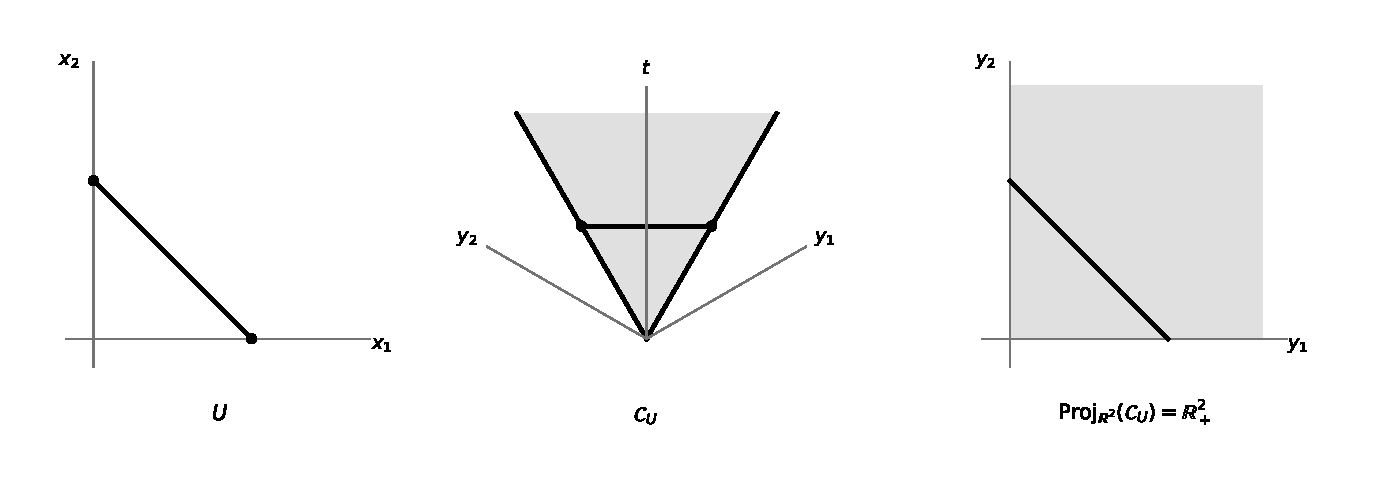
\includegraphics[width=\textwidth]{p4_cone.pdf}}
  {\fbox{\parbox{0.8\textwidth}{\centering \vspace{1em}
   Figure file \texttt{p4\_cone.pdf} not found. Run
   \texttt{p4\_cone.py} in this directory to generate it.
   \vspace{1em}}}}
\caption{Left: $U$, the segment from $(1,0)$ to $(0,1)$. Centre:
$\mathcal{C}_U$ truncated at $t \le 2$. Because $\mathcal{C}_U$ lies in
the plane $y_1 + y_2 = t$ it is flat, so the truncation is the triangle
with apex at the origin and corners $2(1,0,1)$ and $2(0,1,1)$; the dark
segment across it is the slice $t = 1$, which is a copy of $U$. Right:
the projection onto $(y_1,y_2)$, the whole nonnegative orthant, with
$U$ drawn in for comparison. Produced by \texttt{p4\_cone.py}.}
\end{figure}

\subsection*{4.\quad $\Proj_{\mathbb{R}^n}(\mathcal{C}_U) = \cone(U)$
  for any nonempty $U \subseteq \mathbb{R}^n$}

\begin{proposition}
Let $\emptyset \ne U \subseteq \mathbb{R}^n$ and
$\mathcal{C}_U = \{(tx, t) : x \in U,\, t \ge 0\}
 \subseteq \mathbb{R}^n \times \mathbb{R}_+$. Then
\[
  \Proj_{\mathbb{R}^n}(\mathcal{C}_U)
  \;=\; \cone(U) \;=\; \{ t x : x \in U,\; t \ge 0 \}.
\]
\end{proposition}

\begin{proof}
($\subseteq$) Let $y \in \Proj_{\mathbb{R}^n}(\mathcal{C}_U)$. By
definition of the projection there is some $s$ with
$(y, s) \in \mathcal{C}_U$, and by definition of $\mathcal{C}_U$ this
means $(y,s) = (tx, t)$ for some $x \in U$ and $t \ge 0$. Comparing the
first $n$ coordinates gives $y = tx$ with $x \in U$, $t \ge 0$, so
$y \in \cone(U)$.

($\supseteq$) Let $y = tx$ with $x \in U$ and $t \ge 0$. Then
$(y, t) = (tx, t) \in \mathcal{C}_U$ by definition, and projecting
gives $y \in \Proj_{\mathbb{R}^n}(\mathcal{C}_U)$.

Both inclusions hold, so the sets are equal. Nonemptiness of $U$ is used
only to guarantee both sides contain the origin, via $t = 0$.
\end{proof}

Parts 2 and 3 are the instance $n = 2$, $U$ the unit simplex: the
projection came out as $\mathbb{R}^2_+$, which is precisely
$\cone(U)$ for that $U$.

\begin{remark}
Two cautions on the statement.

First, convexity is needed if $\cone(U)$ is read as the \emph{convex}
conic hull. The identity above is about
$\{tx : x \in U,\, t \ge 0\}$, the union of the rays through $U$, which
need not be convex: for $U = \{(1,0),(0,1)\} \subseteq \mathbb{R}^2$ it
is the union of the two axes' nonnegative half-lines, whereas the convex
conic hull is the whole of $\mathbb{R}^2_+$. The two coincide when $U$
is convex.

Second, when $U$ \emph{is} convex, so is $\mathcal{C}_U$. Take
$(t_1x_1, t_1), (t_2x_2, t_2) \in \mathcal{C}_U$ and
$\theta \in [0,1]$, and put $t := \theta t_1 + (1-\theta)t_2$. If
$t > 0$ then
\[
  \frac{\theta t_1 x_1 + (1-\theta) t_2 x_2}{t}
  = \frac{\theta t_1}{t}\,x_1 + \frac{(1-\theta)t_2}{t}\,x_2
\]
is a convex combination of $x_1, x_2$, because the two weights are
nonnegative and sum to $1$; it therefore lies in $U$, and the
combination lies in $\mathcal{C}_U$. If $t = 0$ then
$\theta t_1 = (1-\theta)t_2 = 0$ and the combination is the origin,
which is in $\mathcal{C}_U$. Convexity of $\cone(U)$ then also follows
from Problem 3, Part 2.
\end{remark}

%=======================================================================
\section*{Problem 5.\quad A Minkowski sum \quad[5 pts]}
%=======================================================================

Let $U = \{x \in \mathbb{R}^2 : \|x\|_2 \le 1\}$ and
$V = \{x \in \mathbb{R}^2 : \|x - \mathbf{1}\|_2 \le 1\}$, where
$\mathbf{1} = (1,1)$. Write $B(c, r)$ for the closed Euclidean ball of
centre $c$ and radius $r$, so $U = B(0,1)$ and $V = B(\mathbf{1}, 1)$.

\paragraph{Step 1: scale each ball.} Scaling a ball by
$\alpha > 0$ scales both its centre and its radius, so
\[
  0.5\,U = B(0,\; 0.5),
  \qquad
  0.5\,V = B\big(\tfrac12 \mathbf{1},\; 0.5\big).
\]

\paragraph{Step 2: add two balls.} We claim
$B(c_1,r_1) + B(c_2,r_2) = B(c_1+c_2,\; r_1+r_2)$.

($\subseteq$) If $\|p - c_1\| \le r_1$ and $\|q - c_2\| \le r_2$, then by
the triangle inequality
\[
  \|(p+q) - (c_1+c_2)\| \le \|p - c_1\| + \|q - c_2\|
  \le r_1 + r_2 .
\]

($\supseteq$) Let $\|z - c_1 - c_2\| \le r_1 + r_2$ and set
$d := z - c_1 - c_2$. If $r_1 + r_2 = 0$ the claim is trivial;
otherwise put
\[
  p := c_1 + \frac{r_1}{r_1+r_2}\,d,
  \qquad
  q := c_2 + \frac{r_2}{r_1+r_2}\,d .
\]
Then $\|p - c_1\| = \frac{r_1}{r_1+r_2}\|d\| \le r_1$ and likewise
$\|q - c_2\| \le r_2$, while $p + q = c_1 + c_2 + d = z$.

\paragraph{Step 3: apply it.} With
$c_1 = 0$, $r_1 = 0.5$, $c_2 = \tfrac12\mathbf{1}$, $r_2 = 0.5$,
\[
  \boxed{\;
  0.5\,U + 0.5\,V
  = B\big( \tfrac12 \mathbf{1}, \; 1 \big)
  = \Big\{ x \in \mathbb{R}^2 :
      \big\| x - (\tfrac12, \tfrac12) \big\|_2 \le 1 \Big\}. \;}
\]

So the answer is the unit disk translated to the centre
$(\tfrac12, \tfrac12)$: the \emph{same radius} as $U$, moved to the
midpoint of the two original centres.

\begin{remark}
That the radius does not grow is not an accident of the numbers. Here
$V = U + \mathbf{1}$ is a translate of $U$, so
\[
  0.5U + 0.5V = 0.5U + 0.5U + \tfrac12 \mathbf{1}
              = U + \tfrac12 \mathbf{1},
\]
using $\lambda C + (1-\lambda)C = C$, which holds for every convex $C$
and is just a restatement of convexity. Averaging a convex set with a
translate of itself only translates it.
\end{remark}

%=======================================================================
\section*{Problem 6.\quad A polyhedron in $\mathbb{R}^4$ \quad[20 pts]}
%=======================================================================

\[
  \mathcal{P} := \big\{ (x,y,u,v) \;:\;
    0 \le x \le 1,\; 0 \le y \le 1,\;
    u \ge 0,\; v \ge 0,\; u - v \le 0,\; x + y \le 2 \big\}.
\]
Label the eight rows
\[
  \begin{array}{llll}
  \text{(c1) } x \ge 0, &
  \text{(c2) } x \le 1, &
  \text{(c3) } y \ge 0, &
  \text{(c4) } y \le 1, \\[2pt]
  \text{(c5) } u \ge 0, &
  \text{(c6) } v \ge 0, &
  \text{(c7) } u - v \le 0, &
  \text{(c8) } x + y \le 2 .
  \end{array}
\]
It is useful throughout that $\mathcal{P}$ is a product:
\[
  \mathcal{P} = [0,1]^2 \times Q,
  \qquad
  Q := \{ (u,v) : u \ge 0,\; v \ge 0,\; u \le v \},
\]
because (c8) is implied by (c2) and (c4).

\subsection*{1.\quad Is $\mathcal{P}$ full-dimensional?}

\textbf{Yes, $\dimop \mathcal{P} = 4$.}

It suffices to exhibit an interior point. Take
$(x,y,u,v) = (\tfrac12, \tfrac12, 1, 2)$ and check every row
\emph{strictly}:
\[
  0 < \tfrac12 < 1, \qquad 0 < \tfrac12 < 1, \qquad
  1 > 0, \qquad 2 > 0, \qquad 1 - 2 = -1 < 0, \qquad
  \tfrac12 + \tfrac12 = 1 < 2 .
\]
All eight strict inequalities hold. Since there are finitely many rows
and each is a continuous function, a sufficiently small ball around this
point still satisfies all of them, so $\mathcal{P}$ has nonempty
interior in $\mathbb{R}^4$ and hence $\dimop \mathcal{P} = 4$.

Equivalently one can exhibit five affinely independent points of
$\mathcal{P}$, for instance
\[
  (0,0,0,0),\;(1,0,0,0),\;(0,1,0,0),\;(0,0,0,1),\;(0,0,1,1),
\]
whose four difference vectors from the first are
$e_1, e_2, e_4, e_3 + e_4$, a linearly independent set.

\subsection*{2.\quad The recession cone}

For a polyhedron $\{z : Az \le b\}$ one has
$\rec(\mathcal{P}) = \{d : Ad \le 0\}$: replace every right-hand side by
zero. Doing that row by row:
\[
  \begin{array}{lll}
  \text{(c1)} \Rightarrow d_x \ge 0, &
  \text{(c2)} \Rightarrow d_x \le 0, &
  \text{(c3)} \Rightarrow d_y \ge 0, \\
  \text{(c4)} \Rightarrow d_y \le 0, &
  \text{(c5)} \Rightarrow d_u \ge 0, &
  \text{(c6)} \Rightarrow d_v \ge 0, \\
  \text{(c7)} \Rightarrow d_u - d_v \le 0, &
  \text{(c8)} \Rightarrow d_x + d_y \le 0 . &
  \end{array}
\]
The first pair forces $d_x = 0$ and the second pair $d_y = 0$; (c8) is
then automatic. What remains is $0 \le d_u \le d_v$, in which
$d_v \ge 0$ is implied. Hence
\[
  \boxed{\;
  \rec(\mathcal{P})
  = \big\{ (0,0,d_u,d_v) \;:\; 0 \le d_u \le d_v \big\}
  = \cone\{(0,0,0,1),\,(0,0,1,1)\}. \;}
\]
It is a two-dimensional pointed cone: if $d$ and $-d$ both lie in it
then $d_u \ge 0$ and $-d_u \ge 0$ give $d_u = 0$, and likewise
$d_v = 0$, so it contains no line.

\subsection*{3.\quad Hand computation}

\subsubsection*{(a)\quad All extreme points}

A point of $\mathcal{P} \subseteq \mathbb{R}^4$ is extreme exactly when
the rows active at it have rank $4$.

Because $\mathcal{P} = [0,1]^2 \times Q$, the extreme points are the
pairs of extreme points of the factors. The square $[0,1]^2$ has the
four corners. For $Q$: it is a pointed cone, so its only extreme point
is its apex $(0,0)$. Concretely, if $v > 0$ then at most (c5) or (c7)
can be active, giving rank at most $1$ in the $(u,v)$ block and total
rank at most $3$; the same count rules out $u = v > 0$ and
$0 < u < v$. So $u = v = 0$ at every extreme point.

\[
  \boxed{\;
  \text{Four extreme points: }
  (0,0,0,0),\;\; (0,1,0,0),\;\; (1,0,0,0),\;\; (1,1,0,0). \;}
\]

Rank check at $(0,0,0,0)$: rows (c1), (c3), (c5), (c6) are active with
normals $e_x, e_y, e_u, e_v$, rank $4$. At $(1,1,0,0)$: (c2), (c4),
(c5), (c6) are active, same four normals, rank $4$. The other two are
analogous.

\subsubsection*{(b)\quad All extreme rays}

The extreme rays of $\mathcal{P}$ are the extreme rays of
$\rec(\mathcal{P})$, which from Part 2 is a two-dimensional pointed cone
with exactly two generators:
\[
  \boxed{\; d^1 = (0,0,0,1), \qquad d^2 = (0,0,1,1). \;}
\]

Check that each spans a one-dimensional face, i.e. that the homogeneous
rows active on it have rank $3$. For $d^1$: $d_x = 0$, $d_y = 0$ and
(c5) active ($d_u = 0$); normals $e_x, e_y, e_u$, rank $3$. For $d^2$:
$d_x = 0$, $d_y = 0$ and (c7) active ($d_u = d_v$); normals
$e_x, e_y, e_u - e_v$, rank $3$.

\subsubsection*{(c)\quad All facets}

$\mathcal{P}$ is full-dimensional, so a facet is a face of dimension
$4 - 1 = 3$, and each facet is cut out by exactly one of the given rows
(up to scaling). Taking each row in turn and intersecting:

\begin{center}
\begin{tabular}{@{}llcl@{}}
\toprule
Row & Face $\mathcal{P} \cap \{\text{row tight}\}$ & $\dimop$ & Facet? \\
\midrule
(c1) $x \ge 0$     & $\{0\} \times [0,1] \times Q$ & 3 & yes \\
(c2) $x \le 1$     & $\{1\} \times [0,1] \times Q$ & 3 & yes \\
(c3) $y \ge 0$     & $[0,1] \times \{0\} \times Q$ & 3 & yes \\
(c4) $y \le 1$     & $[0,1] \times \{1\} \times Q$ & 3 & yes \\
(c5) $u \ge 0$     & $[0,1]^2 \times \{(0,v) : v \ge 0\}$ & 3 & yes \\
(c6) $v \ge 0$     & $[0,1]^2 \times \{(0,0)\}$ & 2 & no \\
(c7) $u - v \le 0$ & $[0,1]^2 \times \{(u,u) : u \ge 0\}$ & 3 & yes \\
(c8) $x + y \le 2$ & $\{(1,1)\} \times Q$ & 2 & no \\
\bottomrule
\end{tabular}
\end{center}

Two entries need a word. Setting $v = 0$ in (c6) forces $u = 0$ as well,
through $0 \le u \le v = 0$, which collapses the whole $(u,v)$ block to a
point and leaves dimension $2$. Setting $x + y = 2$ in (c8) forces
$x = y = 1$, since $x \le 1$ and $y \le 1$, leaving $\{(1,1)\} \times Q$
of dimension $2$.

\[
  \boxed{\;
  \text{Six facets: } x \ge 0,\;\; x \le 1,\;\; y \ge 0,\;\;
  y \le 1,\;\; u \ge 0,\;\; u - v \le 0. \;}
\]

\subsubsection*{(d)\quad Which rows are redundant?}

A row is redundant when deleting it leaves $\mathcal{P}$ unchanged. For
a full-dimensional polyhedron the non-redundant rows are exactly the
facet-defining ones, so by (c) the redundant rows are (c6) and (c8), and
each can be seen directly:

\begin{itemize}
  \item \textbf{(c6) $v \ge 0$} follows from (c5) and (c7):
        $v \ge u \ge 0$.
  \item \textbf{(c8) $x + y \le 2$} follows from (c2) and (c4):
        $x + y \le 1 + 1 = 2$.
\end{itemize}

A minimal description is therefore
\[
  \mathcal{P} = \big\{ (x,y,u,v) :
    0 \le x \le 1,\; 0 \le y \le 1,\; 0 \le u \le v \big\},
\]
six inequalities instead of eight.

\subsection*{4.\quad Verification with \texttt{pplpy}}

The script \texttt{p6\_polyhedron.py} builds $\mathcal{P}$ from the
eight given rows and reports the generator and minimal constraint
representations. Its output agrees with the hand computation on every
item:

\begin{center}
\begin{tabular}{@{}lll@{}}
\toprule
Item & By hand & \texttt{pplpy} \\
\midrule
Affine dimension & 4 (full) & 4 \\
Extreme points & the 4 listed in (a) & same 4 \\
Extreme rays & $(0,0,0,1)$, $(0,0,1,1)$ & same 2 \\
Facets & 6 & 6 minimized constraints \\
Redundant rows & (c6), (c8) & (c6), (c8) \\
\bottomrule
\end{tabular}
\end{center}

Redundancy is tested the honest way rather than read off: the script
drops each row in turn, rebuilds the polyhedron and tests it for
equality with $\mathcal{P}$. Only dropping $v \ge 0$ or $x + y \le 2$
leaves the set unchanged.

%=======================================================================
\section*{Problem 7.\quad Dantzig--Wolfe reformulation \quad[15 pts]}
%=======================================================================

\[
\begin{array}{llll}
  \minimize & 3x_1 + 2x_2 + 4y_1 + y_2 & & \\
  \text{s.t.}
    & 2x_1 + x_2 + y_1 + 2y_2 \ge 8, & & \\
    & x_1 + 2x_2 \le 6, & \quad & y_1 - y_2 \le 3, \\
    & 2x_1 + x_2 \le 8, & & y_1 \le 5, \\
    & x_1, x_2 \ge 0, & & y_1, y_2 \ge 0 .
\end{array}
\]

\subsection*{1.\quad The linking constraint and the two blocks}

Only the first row contains both an $x$ and a $y$ variable, so

\[
  \boxed{\;\text{linking constraint: } \;
    2x_1 + x_2 + y_1 + 2y_2 \ge 8. \;}
\]

Every other row involves one block alone, giving

\[
  \mathcal{X} = \big\{ x \in \mathbb{R}^2_+ :
    x_1 + 2x_2 \le 6,\; 2x_1 + x_2 \le 8 \big\},
  \qquad
  \mathcal{Y} = \big\{ y \in \mathbb{R}^2_+ :
    y_1 - y_2 \le 3,\; y_1 \le 5 \big\}.
\]

In the notation used below, $c_x = (3,2)$, $c_y = (4,1)$,
$a_x = (2,1)$, $a_y = (1,2)$ and the right-hand side is $8$.

\subsection*{2.\quad Extreme points and extreme rays of the blocks}

\paragraph{$\mathcal{X}$.} It is bounded: $2x_1 \le 2x_1 + x_2 \le 8$
gives $x_1 \le 4$, and $2x_2 \le x_1 + 2x_2 \le 6$ gives $x_2 \le 3$.
A bounded polyhedron is a polytope, so $\mathcal{X}$ has \emph{no
extreme rays}. Its vertices come from the pairs of tight rows:

\begin{center}
\begin{tabular}{@{}lll@{}}
\toprule
Tight rows & Point & Feasible? \\
\midrule
$x_1 = 0$, $x_2 = 0$ & $(0,0)$ & yes \\
$x_1 = 0$, $x_1 + 2x_2 = 6$ & $(0,3)$ & yes, $2(0)+3 = 3 \le 8$ \\
$x_1 = 0$, $2x_1 + x_2 = 8$ & $(0,8)$ & no, $0 + 16 > 6$ \\
$x_2 = 0$, $x_1 + 2x_2 = 6$ & $(6,0)$ & no, $12 > 8$ \\
$x_2 = 0$, $2x_1 + x_2 = 8$ & $(4,0)$ & yes, $4 + 0 = 4 \le 6$ \\
both slanted rows & $(\tfrac{10}{3}, \tfrac43)$ & yes \\
\bottomrule
\end{tabular}
\end{center}

For the last line, $x_1 = 6 - 2x_2$ substituted into
$2x_1 + x_2 = 8$ gives $12 - 3x_2 = 8$, so $x_2 = \tfrac43$ and
$x_1 = \tfrac{10}{3}$.

\[
  \boxed{\;
  \mathcal{X}: \text{ extreme points }
    (0,0),\;(0,3),\;(\tfrac{10}{3},\tfrac43),\;(4,0);
    \text{ no extreme rays.} \;}
\]

\paragraph{$\mathcal{Y}$.} Its recession cone is
$\{d \ge 0 : d_1 - d_2 \le 0,\; d_1 \le 0\}$, and $d_1 \ge 0$ with
$d_1 \le 0$ forces $d_1 = 0$, leaving $d_2 \ge 0$. So
$\rec(\mathcal{Y}) = \{(0,d_2) : d_2 \ge 0\}$, a single ray:
$\mathcal{Y}$ is unbounded in the $+y_2$ direction. Its vertices:

\begin{center}
\begin{tabular}{@{}lll@{}}
\toprule
Tight rows & Point & Feasible? \\
\midrule
$y_1 = 0$, $y_2 = 0$ & $(0,0)$ & yes \\
$y_2 = 0$, $y_1 - y_2 = 3$ & $(3,0)$ & yes, $3 \le 5$ \\
$y_2 = 0$, $y_1 = 5$ & $(5,0)$ & no, $5 - 0 > 3$ \\
$y_1 = 0$, $y_1 - y_2 = 3$ & $(0,-3)$ & no, $y_2 < 0$ \\
$y_1 - y_2 = 3$, $y_1 = 5$ & $(5,2)$ & yes \\
\bottomrule
\end{tabular}
\end{center}

\[
  \boxed{\;
  \mathcal{Y}: \text{ extreme points }
    (0,0),\;(3,0),\;(5,2);
    \text{ one extreme ray } d = (0,1). \;}
\]

\subsection*{3.\quad The Dantzig--Wolfe reformulation}

\paragraph{Representation.} By Minkowski--Weyl, since $\mathcal{X}$ is a
polytope and $\mathcal{Y}$ is a pointed polyhedron,
\[
  x = \sum_{p \in P_X} \lambda_p\, x^p
  \quad\text{with}\quad \sum_{p \in P_X} \lambda_p = 1,\;\lambda \ge 0,
\]
\[
  y = \sum_{q \in P_Y} \mu_q\, y^q
      + \sum_{r \in R_Y} \nu_r\, d^r
  \quad\text{with}\quad \sum_{q \in P_Y} \mu_q = 1,\;
  \mu \ge 0,\; \nu \ge 0,
\]
where $P_X, P_Y$ index the extreme points and $R_Y$ the extreme ray
found in Part 2. $\mathcal{X}$ contributes no ray variables.

\paragraph{New variables.}
\begin{itemize}
  \item $\lambda_p \ge 0$, $p \in P_X$: the weight placed on extreme
        point $x^p$ of $\mathcal{X}$. Four of them.
  \item $\mu_q \ge 0$, $q \in P_Y$: the weight placed on extreme point
        $y^q$ of $\mathcal{Y}$. Three of them.
  \item $\nu_r \ge 0$, $r \in R_Y$: the multiple of extreme ray $d^r$ of
        $\mathcal{Y}$. One of them, and it is bounded above by nothing.
\end{itemize}

\paragraph{Master problem, in general form.}
\[
\begin{array}{llr}
  \minimize\limits_{\lambda,\mu,\nu} &
    \displaystyle \sum_{p \in P_X} (c_x^{\!\top} x^p)\,\lambda_p
    + \sum_{q \in P_Y} (c_y^{\!\top} y^q)\,\mu_q
    + \sum_{r \in R_Y} (c_y^{\!\top} d^r)\,\nu_r & \\[12pt]
  \text{s.t.} &
    \displaystyle \sum_{p \in P_X} (a_x^{\!\top} x^p)\,\lambda_p
    + \sum_{q \in P_Y} (a_y^{\!\top} y^q)\,\mu_q
    + \sum_{r \in R_Y} (a_y^{\!\top} d^r)\,\nu_r \;\ge\; 8
      & \text{(linking)} \\[12pt]
  & \displaystyle \sum_{p \in P_X} \lambda_p = 1
      & \text{(convexity, } \mathcal{X}) \\[10pt]
  & \displaystyle \sum_{q \in P_Y} \mu_q = 1
      & \text{(convexity, } \mathcal{Y}) \\[8pt]
  & \lambda \ge 0,\;\; \mu \ge 0,\;\; \nu \ge 0 . &
\end{array}
\]

\paragraph{Coefficients for this instance.}

\begin{center}
\begin{tabular}{@{}llrr@{}}
\toprule
Variable & Generator & Objective cost & Linking coefficient \\
\midrule
$\lambda_1$ & $x^1 = (0,0)$ & $0$ & $0$ \\
$\lambda_2$ & $x^2 = (0,3)$ & $6$ & $3$ \\
$\lambda_3$ & $x^3 = (\tfrac{10}{3},\tfrac43)$
            & $\tfrac{38}{3}$ & $8$ \\
$\lambda_4$ & $x^4 = (4,0)$ & $12$ & $8$ \\
$\mu_1$     & $y^1 = (0,0)$ & $0$ & $0$ \\
$\mu_2$     & $y^2 = (3,0)$ & $12$ & $3$ \\
$\mu_3$     & $y^3 = (5,2)$ & $22$ & $9$ \\
$\nu_1$     & $d^1 = (0,1)$ & $1$ & $2$ \\
\bottomrule
\end{tabular}
\end{center}

For instance $c_x^{\!\top} x^3 = 3(\tfrac{10}{3}) + 2(\tfrac43)
= 10 + \tfrac83 = \tfrac{38}{3}$ and
$a_x^{\!\top} x^3 = 2(\tfrac{10}{3}) + \tfrac43 = 8$, while for the ray
$c_y^{\!\top} d^1 = 1$ and $a_y^{\!\top} d^1 = 2$.

\paragraph{Master problem, written out.}
\[
\begin{array}{ll}
  \minimize &
    6\lambda_2 + \tfrac{38}{3}\lambda_3 + 12\lambda_4
    + 12\mu_2 + 22\mu_3 + \nu_1 \\[4pt]
  \text{s.t.} &
    3\lambda_2 + 8\lambda_3 + 8\lambda_4
    + 3\mu_2 + 9\mu_3 + 2\nu_1 \;\ge\; 8, \\[2pt]
  & \lambda_1 + \lambda_2 + \lambda_3 + \lambda_4 = 1, \\[2pt]
  & \mu_1 + \mu_2 + \mu_3 = 1, \\[2pt]
  & \lambda, \mu, \nu \ge 0 .
\end{array}
\]

Eight variables and three rows, against four variables and five rows in
the original. That is the characteristic trade of Dantzig--Wolfe: the
block rows disappear into the generator description and are replaced by
one convexity row per block, at the price of a variable per generator,
which is why the method is normally run with column generation rather
than by listing all generators as here.

\paragraph{Recovering a solution.}
$x = \sum_p \lambda_p x^p$ and
$y = \sum_q \mu_q y^q + \sum_r \nu_r d^r$.

\paragraph{Check.} Solving both programs exactly over the rationals
gives the same optimal value $4$: the master picks
$\lambda_1 = 1$, $\mu_1 = 1$, $\nu_1 = 4$, which recovers
$x = (0,0)$ and $y = (0,0) + 4(0,1) = (0,4)$, matching the optimal
solution of the original problem. The ray is what makes this cheap: it
buys $2$ units of the linking row per unit of cost, against $1.5$ for
the best extreme point, and nothing bounds $\nu_1$ from above.

%=======================================================================
\vspace{1em}
\hrule
\vspace{0.6em}
{\small Problems 1, 2, 3, 5 and 7 are proofs and hand computations.
\texttt{p4\_cone.py} produces the Problem 4 figure and checks the
projection with \texttt{pplpy}; \texttt{p6\_polyhedron.py} answers
Problem 6 Part 4; \texttt{p7\_dantzig\_wolfe.py} is an extra check that
solves the original program and the master exactly over the rationals
and confirms they agree. The code verifies the hand results and does not
replace them.}

\end{document}
